
% Chapter One
%

\chapter{INTRODUCTION}

\section{Stellar Nucleosynthesis}
Nuclear astrophysics is an interdisciplinary field of science that includes the macroscopic world of astrophysics and the microscopic world of nuclear physics.  In other words, nuclear reactions in stars control the stellar evolution microscopically, while the stellar evolution restricts the nuclear reactions on a macroscopic scale.
 % The study can be tracked back to about 100 years ago, when Eddington proposed that the source energy in the Sun comes from its internal hydrogen fusion into Helium in 1920[1].
%%%


 At the beginning of the stellar evolution of a single star, there is only an interstellar gas cloud consisting of hydrogen, helium and a small amount of other light elements after the Big Bang. The gas collapses gravitationally, increasing the thermal energy that heats up the system. The fates of stars diverge based on their mass:  if the mass of the system is M $\lesssim$ 0.08M$_\odot$, where M$_\odot$ is the solar mass, the central temperature is not high enough to initiate nuclear reactions. Lives of these protostars then end up as brown dwarf stars.  On the contrary, those with masses of M $\gtrsim$ 0.08M$_\odot$ can reach the temperature in their cores to  T $\sim$ $10^7$ K, igniting  the hydrogen burning that fuses hydrogen to helium (4p $\rightarrow$ $^4$He) in the core and releases nuclear energy that  prevents further gravitational contraction. Depending on their initial mass and composition, the hydrogen burning proceeds through pp chains for stars with mass M $\lesssim$ 1.5M$_\odot$, or mainly via CNO cycle for M $\gtrsim$ 1.5M$_\odot$.  Stars that achieve hydrostatic equilibrium by  hydrogen burning, like the Sun, are called main-sequence stars and they stay in this stage for most of their lives. The theory of the energy source of the Sun was discovered by Bethe $et\ al.$~\citep{Bethe1939}, and he was awarded the Nobel Prize in Physics in 1967. It is known that the Sun can burn its core hydrogen for 10 Gy and it has been burning for 4.5 Gy.

When stars run out of most of the hydrogen in the center, the nuclear process can no longer provide enough energy to prevent the gravitational collapse. For stars with M $\lesssim$ 0.4M$_\odot$, the core contracts until  electron degeneracy sets in. They slowly achieve  equilibrium  and become  helium dwarfs. On the other hand,  the temperature of stars  with  M $\gtrsim$ 0.4M$_\odot$ can  reach  0.1 GK where the helium burning ignites, resulting in stars that leave the main sequence and develop into red giants.  In the center helium fuses to carbon and oxygen by the so-called 3-$\alpha$ process ($\alpha + \alpha \rightleftharpoons$ $^8$Be $\rightarrow + \alpha$ $^{12}$C) and $^{12}$C($\alpha$, $\gamma$)$^{16}$O.


If the mass of stars is large enough (M $\gtrsim$ 8M$_\odot$), the burning phase can proceed to the next stage, i.e. the carbon-burning phase, when the helium is exhausted in the core and the  center temperature reaches 1 GK. Otherwise stars with the mass of M $\lesssim$ 8M$_\odot$ will gradually cool down as white dwarfs.  In the next burning phase, heavy charged particle reactions take place in the sequence of carbon-, neon-, oxygen- and silicon-burning, converting the core to heavier nuclei up to A $\sim$ 60. At this point the structure of such stars just before the final stage presents an `onion-like' structure. When a more advanced burning phase ignites, the previous burning may not completely disappear, but still take place in a shell surrounding the core (See Fig.\ref{fig:onion}). The iron core grows as the shell keeps burning. This process continues until the point where the electron degeneracy fails to counteract  gravity, the core collapses rapidly and the star turns into a Type II supernova, releasing an explosively  large amount of energy and nucleosynthesis products in the ejected shell into  space. The leftover of the core will become a neutron star or a black hole depending on the mass of the star.



%%%Concretely, nuclear reactions in stars control the the stellar evolution microscopically, while the stellar evolution restricts the nuclear reactions in the macroscopic scale. In the eye of the stellar evolution of single stars, in the beginning there are only
%%%
%%%
%%%

It is known that the nucleosynthesis of the two lightest elements, hydrogen and helium took place shortly after the Big Bang. All other light isotopes below iron (A $\sim$ 60) are induced by charged particle reactions. However,  for nuclei with mass larger than the mass of iron, charged particle reactions are less likely to create heavier elements due to the increasing Coulomb repulsion. For this reason, neutron capture reactions are believed to be the most effective pathway for creating elements beyond iron. The theory and experimental studies were first published by Margaret Burbidge, Geoffrey Burbidge, William Fowler and Fred Hoyle, known as B$^2$FH paper in 1957~\citep{B2FH} and William Fowler wins the Nobel Prize in Physics in 1983.

There are two types of neutron capture processes based on the rate of neutron capture compared to the $\beta$-decay lifetime of the nuclei produced. In case of the rapid neutron capture process ($r$-process), the neutron capture rate is faster than the $\beta$-decay lifetime whereas for the slow process ($s$-process) the neutron capture is slower than the corresponding $\beta$-decay rate.
The classical approach for the $s$-process model shows that the observed $s$-process abundances
could be reproduced successfully with three different exponential distribution of neutron exposures, that one set was needed with lower exposure (called $weak$ component,  $N_n \textless 10^8$ cm$^{-3}$ where $N_n$ refers to the neutron density) and on with higher (called $main$ component, $N_n \sim 10^8$ $cm^{-3}$ ). The last component, the $strong$ component, is not the critical topic in this work as it is only necessary to explain the abundance maximum at $^{208}$Pb.~\citep{Kappeler1989}%[Kaeppeler et al. 1989].


The $main$ component of the $s$-process has been seen in the low mass Asymptotic Giant Branch (AGB) stars (1M$_{\odot}<$  M $<$ 4M$_{\odot}$) during the helium shell burning at $T_9 \sim$ 0.1 GK, where the  $^{13}$C($\alpha$,n)$^{16}$O reaction serves as the dominant
neutron source. It is responsible for producing elements
in the range of 90 $\leq$ A $\leq$ 209. On the contrary, the weak component of the  $s$-process
synthesizes elements from 60 $\leq$ A $\leq$ 90 and is likely to take
place at the end of helium and carbon burning in massive stars (M $>$ 10M$_{\odot}$) at a higher temperature ($T_9 \sim$ 0.3 GK).
The dominant reaction that provides neutrons
for the weak $s$-process is the $\alpha$-capture reaction on
$^{22}$Ne through the reaction sequence
$^{14}$N($\alpha$,$\gamma$)$^{18}F$($\beta$,$v$)$^{18}$O($\alpha$,$\gamma$)$^{22}$Ne($\alpha$,n)$^{25}$Mg, where $^{14}$N is the leftover of the CNO cycle. The present work focuses  mainly on the neutron sources for the weak component of the $s$-process.
\begin{figure}[tpb]
  \begin{center}
    \centerline{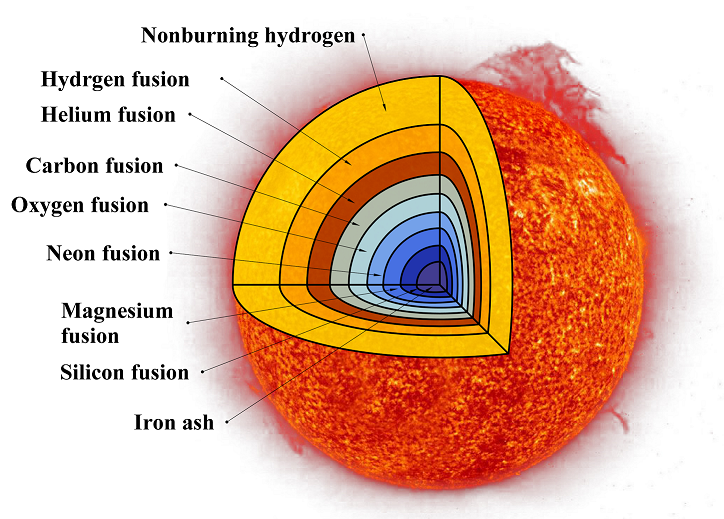
\includegraphics[scale=0.6]{graph/ch1/onion_1}}
    \caption{Onion-like structure just before the end of the life for a massive star.}
    \label{fig:onion}
  \end{center}
\end{figure}

The nuclear reactions are not only the main energy sources that act against the gravitational contraction of stars, but also the only mechanism by which all isotopes  except for hydrogen are synthesized in the universe. The production of energy and elements by nuclear processes, in turn, explains the structure and evolution of the universe. Stellar nucleosynthesis is therefore a  critical topic that focuses on how elements are produced in the universe and its influence on star evolution. For the understanding of the past and the present, as well as to make predictions for the development of the universe, it is, therefore, essential to fully understand the synthesis of the elements in our universe.


\section{The $s$-process components}

As mentioned in the last section,  nuclei heavier than iron (A $\textgreater$ 56) are mainly synthesized by processes involving the neutron capture (i.e. the neutral-particles capture) on preformed seed nuclei instead of charged particle reactions. This is due to the fact that the temperature required to produce enough energy for charged particle reactions to overcome the rapidly rising Coulomb barriers of the heavy nuclides would be so high that they would destroy those seed nuclei through photonuclear reactions\citep{Boyd}.%[R. Boyd]


\begin{figure}[tpb]
  \begin{center}
    \centerline{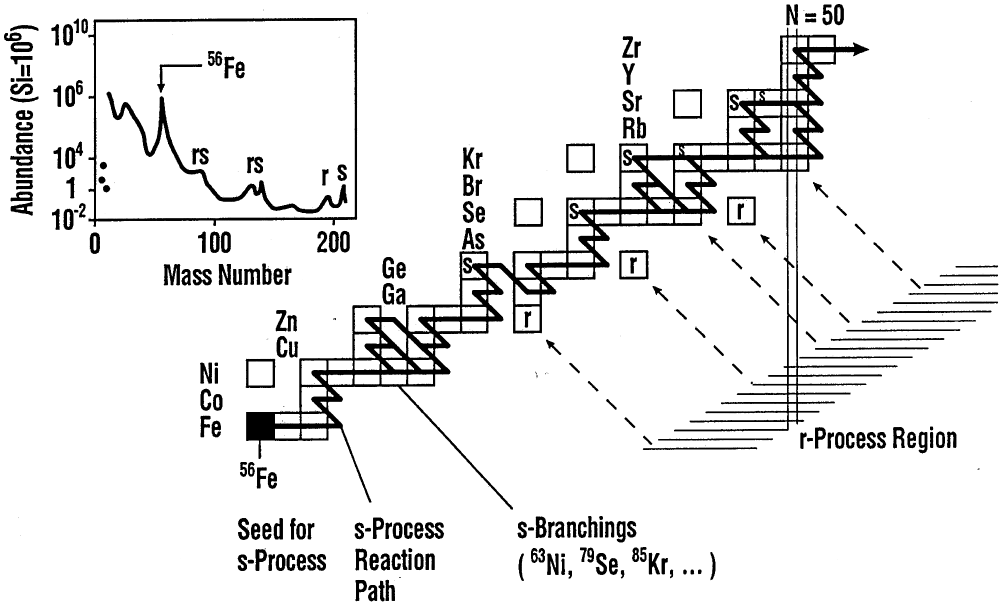
\includegraphics[scale=0.5]{graph/ch1/n-cap}}
    \caption{Chart of the nuclides showing the path of the s-process starting from  iron~\citep{Kappeler2011}. See retails in the text.}
    \label{fig:n-cap}
  \end{center}
\end{figure}

The s-process proceeds through nuclei that $\beta$-decay rapidly compared with the time between successive neutron capture.  It starts from the iron seed along the group of stable nuclei and will eventually terminate at the most massive stable nucleus $^{209}$Bi. Fig.~\ref{fig:n-cap} illustrated the path of the s-process in a portion of the chart of the nuclides, along with the r-process which  drives the nuclei to the neutron-rich region. 
The inset gives the solar abundance distribution relative to 10$^6$ Si atoms. The sharp abundance peaks denoted as $s$  near the mass numbers A = 88, 138 and 208 (corresponding to the neutron magic numbers of N = 50, 82 and 126, respectively) are due to the s-process,  indicating  the impact of the nuclear structure effect.
The s-process can be considered as a ��secondary�� process
in the sense that the seed nuclei (typically $^{56}$Fe) must have existed at the stellar birth as the stellar evolution does not produce the heavy elements before those burning phases are triggered. This is in contrast to  the r-process which generally is referred to as a `primary' process as it is likely to proceed on freshly produced seeds in the interiors of extreme stellar environment (Type-II supernovae for instance).


%%%%%


According to the classical approach to describe s-process model\citep{Kappeler1989}\citep{CLAYTON1961}, under neutron irradiation, for an  isotope A the change in abundance ($N_s(A)$) with time  can be written as
 \begin{equation}
    \label{Na_rate}
    \begin{aligned}
        dN_s(A)/dt = \lambda_n(A-1)N_s(A-1) - (\lambda_n(A) + \lambda_{\beta}(A)) N_s(A)
    \end{aligned}
\end{equation}
where the neutron capture rate $\lambda_n$ is proportional to the neutron capture cross section $\sigma$ and the neutron flux $\Phi$ by $\lambda_n = \sigma \Phi$. The neutron flux $\Phi$ is the product of neutron density $n_n$ and the thermal neutron velocity $v_T = (2kT/m)^{1/2}$, where $m$ refers to the reduced mass. The $\beta$-decay rate $\lambda_\beta=\ln 2/t_{1/2}$ for a radioactive isotope A.

With two assumptions in the classical model: (i)The s-process temperature $T$ is constant as the neutron capture rates are almost independent of  temperature and (ii) The radioactive nuclei on the synthesis path is stable ($\lambda_\beta \ll \lambda_n$), Eq~\ref{Na_rate} can be rewritten by the time-integrated neutron flux $\tau = \int \Phi dt$,
 \begin{equation}
    \label{Na_rate2}
    \begin{aligned}
        dN_s(A)/d\tau = \sigma(A-1)N_s(A-1)-\sigma(A)N_s(A)
    \end{aligned}
\end{equation}
When the system reaches the equilibrium, the production and destruction terms in Eq.\ref{Na_rate2} leading to a constant product of cross section and s-process abundance, written as $\sigma N_s$. $\sigma N_s$ is the characteristic quantity of the classical s-process.

As the abundances of s-only isotopes cannot only be reproduced by a single irradiation of an iron seed\citep{CLAYTON1961}, the assumption that the neutron exposure was in the form of   an exponential distribution\citep{SeegerP1965}, written as
 \begin{equation}
    \label{rho}
    \begin{aligned}
        \rho(\tau) = \frac{f N_{56}}{\tau_0} \exp(-\tau/\tau_0),
    \end{aligned}
\end{equation}
where $\rho$ represents the fraction of iron seeds that have been irradiated in a unit time. $\tau_0$ refers to the mean neutron exposure,  $N_{56}$ is  the number of irradiated iron seeds and $f$ is the fraction of the number of the iron nuclei.

Eq.\ref{rho}  leads to the  solution of the system of Eq.~\ref{Na_rate2}
 \begin{equation}
    \label{product}
    \begin{aligned}
    \sigma(A)N_s(A) = \frac{f N_{56}}{\tau_0} \prod^A_{i=56}[1+(\sigma(i)\tau_0)^{-1}]^{-1}
    \end{aligned}
\end{equation}

% EXplain the measured data point in Fig.2
As mentioned in the last section, according to the phenomenological s-process model analysis for Eq.~\ref{product}~\citep{Kappeler1989}~\citep{CLAYTON1961}, there are three distinct components are needed to  fit the solar abundance distribution of the s-process elements, which is described by the $N_{s}(A) \langle \sigma_s \rangle $ curve as a function of neutron exposure. Fig.~\ref{fig:abundance} shows the clear separation of the two s-process components, the weak component and the main component, by depicting the cross section times the s-process abundance ($N_{s}(A) \langle \sigma_s \rangle $) as a function of the mass number. The measured data points correspond to the experimental measurement for the s-only nuclei. The thick solid line represents the  main component calculated from the means of the classical model, which fits the measured data well especially for nuclei with large mass numbers. The thin solid line refers to the result of the weak component in  massive stars, which is successful in describing s-process products with mass number up to A = 90.
%One should also notice that at A = 84, 138 and 208 the cross sections for
%neutron captures into new neutron shells are very small since these nuclei correspond
%to magic neutron numbers N = 50, 82 and 126, respectively. Therefore, for a given
%supply of neutrons, the  product drops to a new plateau as shown in Figure\ref{fig:abundance}.

%State that 3 components are needed to fit the data(thin line)


%Introduce those 3 components

\begin{figure}[tpb]
  \begin{center}
    \centerline{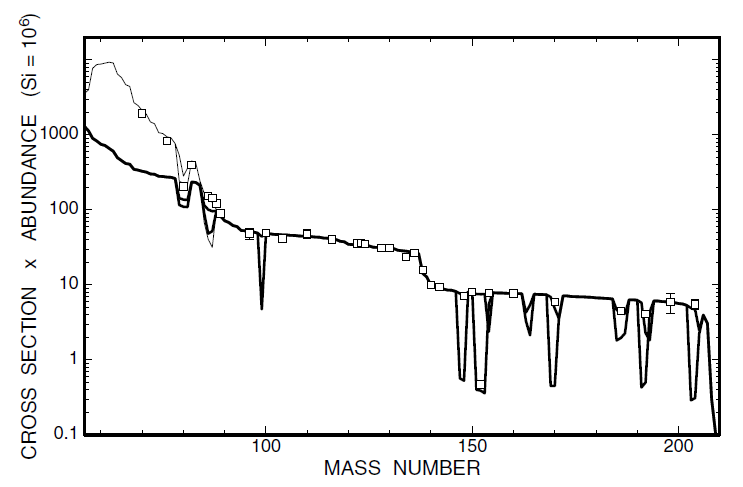
\includegraphics[scale=0.6]{graph/ch1/abundence}}
    \caption{The product of the cross section and the s-process abundance v.s. the mass number. The thin line refers to the weak component in massive stars obtained by means of the classical model and the thick line represents the main component. The  data points denote the experimental results for the s-only nuclei. Figure from Ref.~\citep{Kappeler2011}}
    \label{fig:abundance}
  \end{center}
\end{figure}

%%%%

It is reasonable to assume that different sites are required for each of the observed s-process components. The astrophysics sites for main- and weak- components are described in the following subsections.


\subsection{AGB stars}

The main component of the s-process is shown to occur in low mass as well as intermediate mass (0.8M$_\odot$ $\lesssim$ M $\lesssim$ 8M$_\odot$ ) Asymptotic Giant Branch (AGB) stars during a thermal pulsing phase, accounting for the s-process nuclei in the mass range  90 $\lesssim$ A $\lesssim$ 208.  The model of an AGB star can be explained by the evolution of M = 5$M_{\odot}$ in  the Hertzsprung-Russel (HR) diagram, which plots the luminosity versus surface temperature of a star (shown in Fig.~\ref{fig:AGB}).

Core hydrogen burning sets in on the zero age main sequence (ZAMS) and   slowly continues,  converting hydrogen in its core into helium. Once a significant fraction of about 10$\%$ of central hydrogen is exhausted, which takes about 10$^9$ to 10$^{10}$ years, the star will move towards the red giant phase as the envelope expands. Between the first dredge-up and the red giant branch (RGB), the hydrogen shell burns  and brings helium to the core, increasing the temperature rapidly, therefore, the core helium burning is ignited. The envelope expands once again as the core burns its helium until the core helium runs of out of materials. At this point the hydrogen and helium shell will burn periodically around the C-O core. The star will then undergo a thermal pulsing (TP) AGB phase, where the helium shell surrounding the C-O core and the hydrogen in the outer convective shell  burn alternately. At this moment the star appears close to the RGB, giving the name of AGB phase.


\begin{figure}[tpb]
  \begin{center}
    \centerline{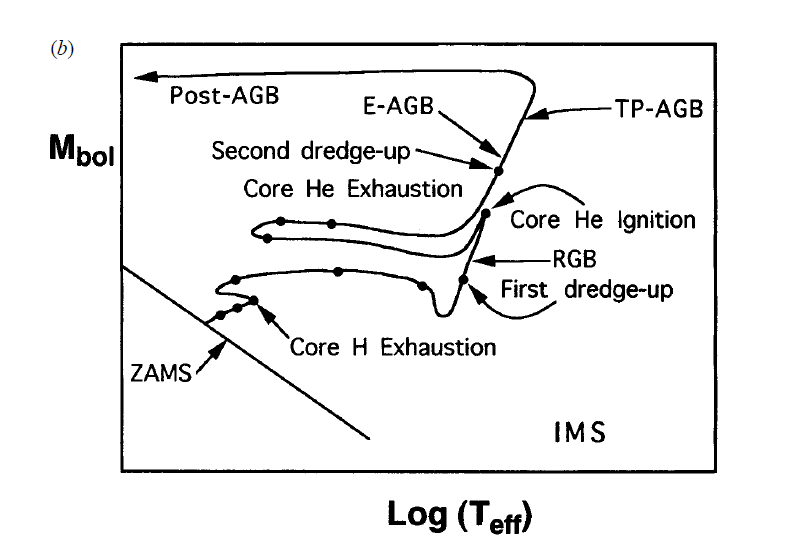
\includegraphics[scale=0.6]{graph/ch1/AGB_HR}}
    \caption{HR diagram for a AGB star (M = 5 M$_\odot$).}
    \label{fig:AGB}
  \end{center}
\end{figure}

During the AGB phase, after the quiescent of a TP, the convective envelope penetrates below the hydrogen shell and the helium shell, mixing the carbon and oxygen into the intershell, and adds a small amount of protons into the top layer of the helium from the hydrogen shell. The protons then can be captured by $^{12}$C through the reaction $^{12}$C(p,$\gamma$)$^{13}$N($\beta^+v$)$^{13}$C, producing a so-called $^{13}$C pocket. The $^{13}$C is consumed in the helium intershell in the AGB phase before a new TP develops. This is the dominant neutron source for the main s-process component.

\subsection{Massive stars}

Another s-process site, the weak $s$-process component is thought to originate mainly from the core helium burning stage in massive stars (M $\gtrsim$ 13M$_\odot$) during the pre-supernovae evolution, producing light s-elements in the A $\sim$ 60 - 90 mass range.

At the beginning of the helium burning in the core, the $^{14}$N produced by the preceding CNO cycles during the hydrogen burning phase are rapidly converted to $^{22}$Ne by successive $\alpha$ captures and a $\beta$-decay through  $^{14}$N($\alpha$,$\gamma$)$^{18}$F($\beta ^{+} v$) $^{18}$O($\alpha,\gamma$)$^{22}$Ne. Towards the end of the helium burning when most of the helium is exhausted (about 10$\%$ left), when the temperature reaches $\sim$ 2.5 GK, the $^{22}$Ne($\alpha$,n)$^{25}$Mg neutron source becomes operative. The remaining $^{22}$Ne left over from helium burning is the main neutron source during the subsequent carbon shell burning. This process is sensitive to the treatment of mixing at the edge of the convective zone during the end of the core helium burning.


%The main neutron source triggering the s-process in massive stars is the 22Ne(a,n) reaction.




\section{Astrophysical Importance of the $^{25}$Mg(d,p)$^{26}$Mg}


So far it is known that $^{22}$Ne($\alpha$,n)$^{25}$Mg is the main neutron source for the  weak s-process component in massive stars during core helium burning and in AGB stars during helium-shell burning. Most of the neutrons are captured by various neutron poisons, especially by $^{25}$Mg since it has a very large neutron capture cross sections, therefore dramatically reducing the number of neutrons per $^{56}$Fe seed. The competing reaction  $^{22}$Ne($\alpha$,$\gamma$)$^{26}$Mg is another neutron poison, since the cross sections of both reactions are  dominated by the contribution of low energy and natural parity resonances\citep{Kappeler2011}. Considerable effort has been made in the past to measure the low energy resonances in $^{22}$Ne($\alpha$, $\gamma$) and $^{22}$Ne($\alpha$, n) \citep{Wolke1989}\citep{Jaeger2001}to determine their impact on the channel branching and the overall efficiency of the neutron sources in the stellar environment. There are a number of low energy resonances which have not yet been measured because of the extremely small cross sections. Only limited experimental information is available about these states in the compound nucleus $^{26}$Mg which primarily results from transfer reactions, neutron capture or photo-excitation studies. This lack of information introduces considerable uncertainties into the calculation of the reaction rates and can have an significant influence on the calculated nucleosynthesis in massive stars.


The lowest-lying known resonance in the $^{22}$Ne + $\alpha$  channel has been observed at a center of mass energy of E$\alpha$ = 703 keV corresponding to an excitation energy in $^{26}$Mg of 11.318 MeV \citep{Wolke1989}\citep{Jaeger2001}. Additional 38 states have been reported between the alpha threshold at 10.615 MeV and this resonance, which might contribute to the stellar-reaction rate. 16 of these states are above the neutron threshold of E$\alpha$ = 478 keV (E$x$ =11.093 MeV) and can contribute to both the ($\alpha$,n)- and the ($\alpha$, $\gamma$)-reaction channel. The actual number of relevant states will be lower because only natural parity states can be populated in the  $^{22}$Ne + $\alpha$ system.

Since the ($\alpha$,n) and the ($\alpha$, $\gamma$) reaction are competing with each other, it is necessary to know the ratio of the  gamma to neutron width, $\Gamma_{\gamma}/\Gamma_{n}$.
The role of the $^{22}$Ne($\alpha$,n) reaction as a stellar neutron source might be impacted if the stellar-reaction rate for $^{22}$Ne($\alpha$, $\gamma$) reaches a few percent of the $^{22}$Ne($\alpha$,n) reaction. Detailed information is available about neutron-unbound states within the first 500 keV above the neutron threshold from (n,$\gamma$) experiments~\citep{Massimi}~\citep{Koehler2002}. These two experiments provide precise excitation energies and determine the $\gamma$ and neutron widths for these states with ratios $\Gamma_{\gamma}/\Gamma_{n}$ ranging from 10$^{-4}$ to 10. However they failed to observe the 703 keV resonance which has been observed in both reactions. In addition, the (n,$\gamma$) experiments mainly populate s- and p-wave resonances and definite spin and parity assignments were not possible for a majority of the observed states.

To clarify the situation we propose a high resolution measurement of the $^{25}$Mg(d,p)$^{26}$Mg
reaction to populate states within 1 MeV above the alpha threshold using the Grand Raiden Spectrometer at the Research Center for Nuclear
Physics (RCNP) in Osaka, Japan. The goals of  the experiment are (i) Precise measurement of excitation energies; (ii) Restricting spin and parity of observed states; (iii) Observation of the 11.32 MeV state which is missing in the n-ToF measurement; (iv) Determination of the neutron spectroscopic factors.

% % uncomment the following lines,
% if using chapter-wise bibliography
%
% \bibliographystyle{ndnatbib}
% \bibliography{example}
